
\begin{frame}{Compute graph}
	\begin{block}{ Partial derivatives of $f(x,y,z)= sin(x^2y)+e^z$}
		\begin{align}
			\frac{\partial f}{\partial x} &= 2xycos(x^2y) \\
			\frac{\partial f}{\partial y} &= x^2cos(x^2y) \\
			\frac{\partial f}{\partial z} &= e^z 
		\end{align}
	\end{block}
\end{frame} 

\begin{frame}{Compute graph}
	\begin{block}{ Compute graph of $f(x,y,z)= sin(x^2y)+e^z$}
		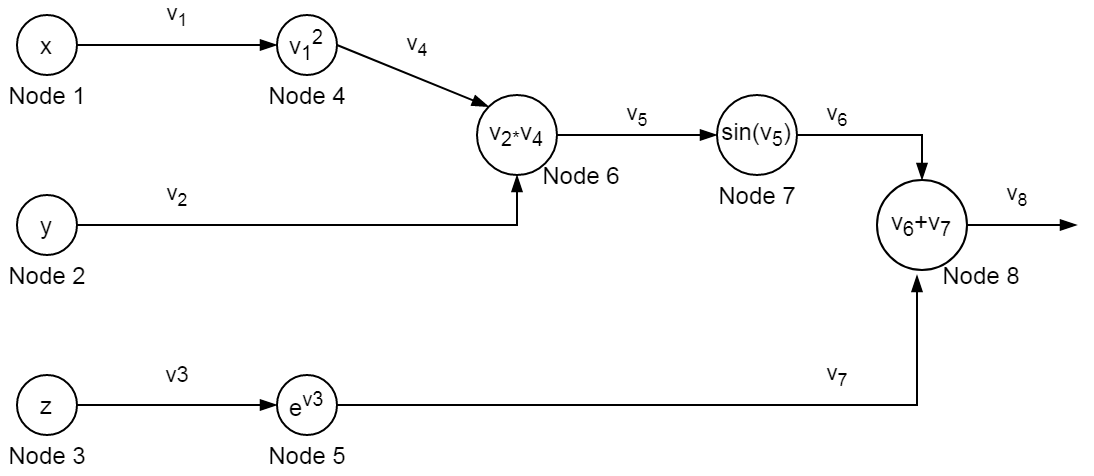
\includegraphics[width=1.\textwidth, center]{figuras/backprop_eg1.png}
	\end{block}
\end{frame}

\begin{frame}{}
	\begin{columns}[T]
		\begin{column}{.5\textwidth}
			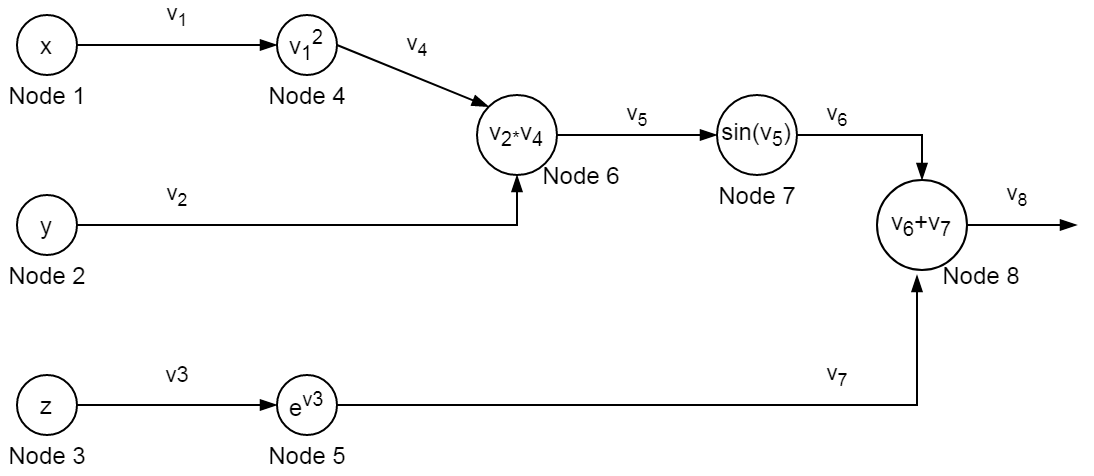
\includegraphics[width=1.1\textwidth, center]{figuras/backprop_eg1.png}
			%{\tiny 
			\begin{align*}
					\frac{\partial v_8}{\partial z}&= 
					\frac{\partial v_8}{\partial v_7} 
					\frac{\partial v_7}{\partial v_3} 
					\frac{\partial v_3}{\partial z}  \\
					&= 1.e^{v_3}.1 \\
					\frac{\partial v_8}{\partial z}&=\frac{\partial f}{\partial z} 
					= e^{v_3}=e^z 
			\end{align*}
			%}
		\end{column}
		\begin{column}{.5\textwidth}
			\begin{align*}
			\frac{\partial v_8}{\partial y}&= 
			\frac{\partial v_8}{\partial v_6} 
			\frac{\partial v_6}{\partial v_5} 
			\frac{\partial v_5}{\partial v_2}  
			\frac{\partial v_2}{\partial y}\\
			& = 1.cos(v_5).v^4.1 \\
			\frac{\partial f}{\partial y}&=\frac{\partial v_8}{\partial y}
			= cos(v_5)v^4 \\
			&= cos(v_2v_4)v_4 \\
			&= cos(v^2_1y)v^2_1 \\
			&= cos(x^2y)x^2
			\end{align*}
		\end{column}
	\end{columns}
\end{frame}